\documentclass[border=6pt]{standalone}
\usepackage{tikz}
\usetikzlibrary{arrows.meta,positioning,calc,shapes.geometric,fit,backgrounds,patterns,matrix,decorations.pathreplacing}
\begin{document}
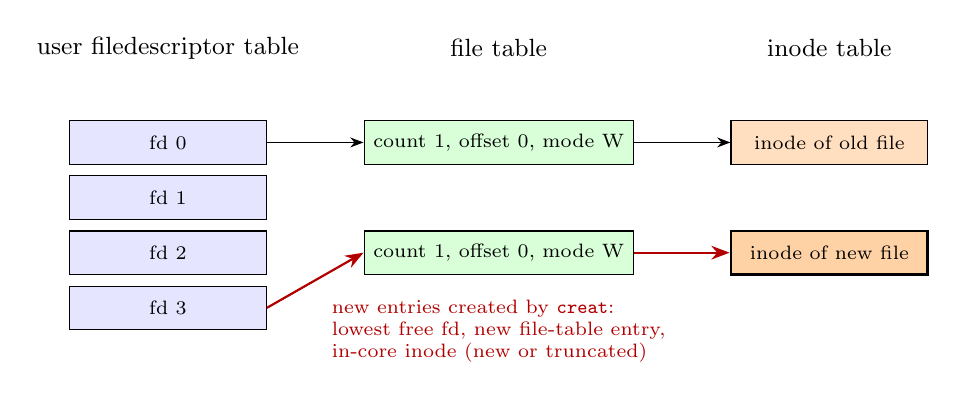
\begin{tikzpicture}[>=Stealth,font=\small]
\tikzstyle{b}=[draw,minimum height=0.55cm,minimum width=2.5cm,font=\scriptsize]
\node[font=\small] at (0,1.2) {user file\\ descriptor table};
\node[font=\small] at (4.2,1.2) {file table};
\node[font=\small] at (8.4,1.2) {inode table};
\foreach \i in {0,1,2,3} \node[b,fill=blue!10] (u\i) at (0,-\i*0.7) {fd \i};
\node[b,fill=green!15,minimum width=3.0cm] (f0) at (4.2,0) {count 1, offset 0, mode W};
\node[b,fill=green!15,minimum width=3.0cm] (f1) at (4.2,-1.4) {count 1, offset 0, mode W};
\node[b,fill=orange!25] (i0) at (8.4,0) {inode of old file};
\node[b,fill=orange!35,line width=1pt] (i1) at (8.4,-1.4) {inode of new file};
\draw[->] (u0.east) -- (f0.west);
\draw[->,thick,red!70!black] (u3.east) -- (f1.west);
\draw[->] (f0.east) -- (i0.west); \draw[->,thick,red!70!black] (f1.east) -- (i1.west);
\node[font=\scriptsize,red!70!black,align=left] at (4.2,-2.4) {new entries created by \texttt{creat}:\\ lowest free fd, new file-table entry,\\ in-core inode (new or truncated)};
\end{tikzpicture}
\end{document}
